\subsection{Effet de l'aphasie de Broca sur la qualité de vie}

Il n'est pas surprenant que l'aphasie ait un impact négatif sur la qualité de vie des individus qui en souffrent.
En effet, les individus atteints d'aphasie ont une moins bonne qualité de vie que les individus en bonne santé
selon les critères WHOQOL-BERF\footnote{\citeurl{WHOQOL}} 
et WPI\footnote{\citeurl{WPI}}(voir Table~\ref{tab.qol-compare},\barecite{Ross_Wertz_2010}).

\begin{table}[hbt]
    \centering
    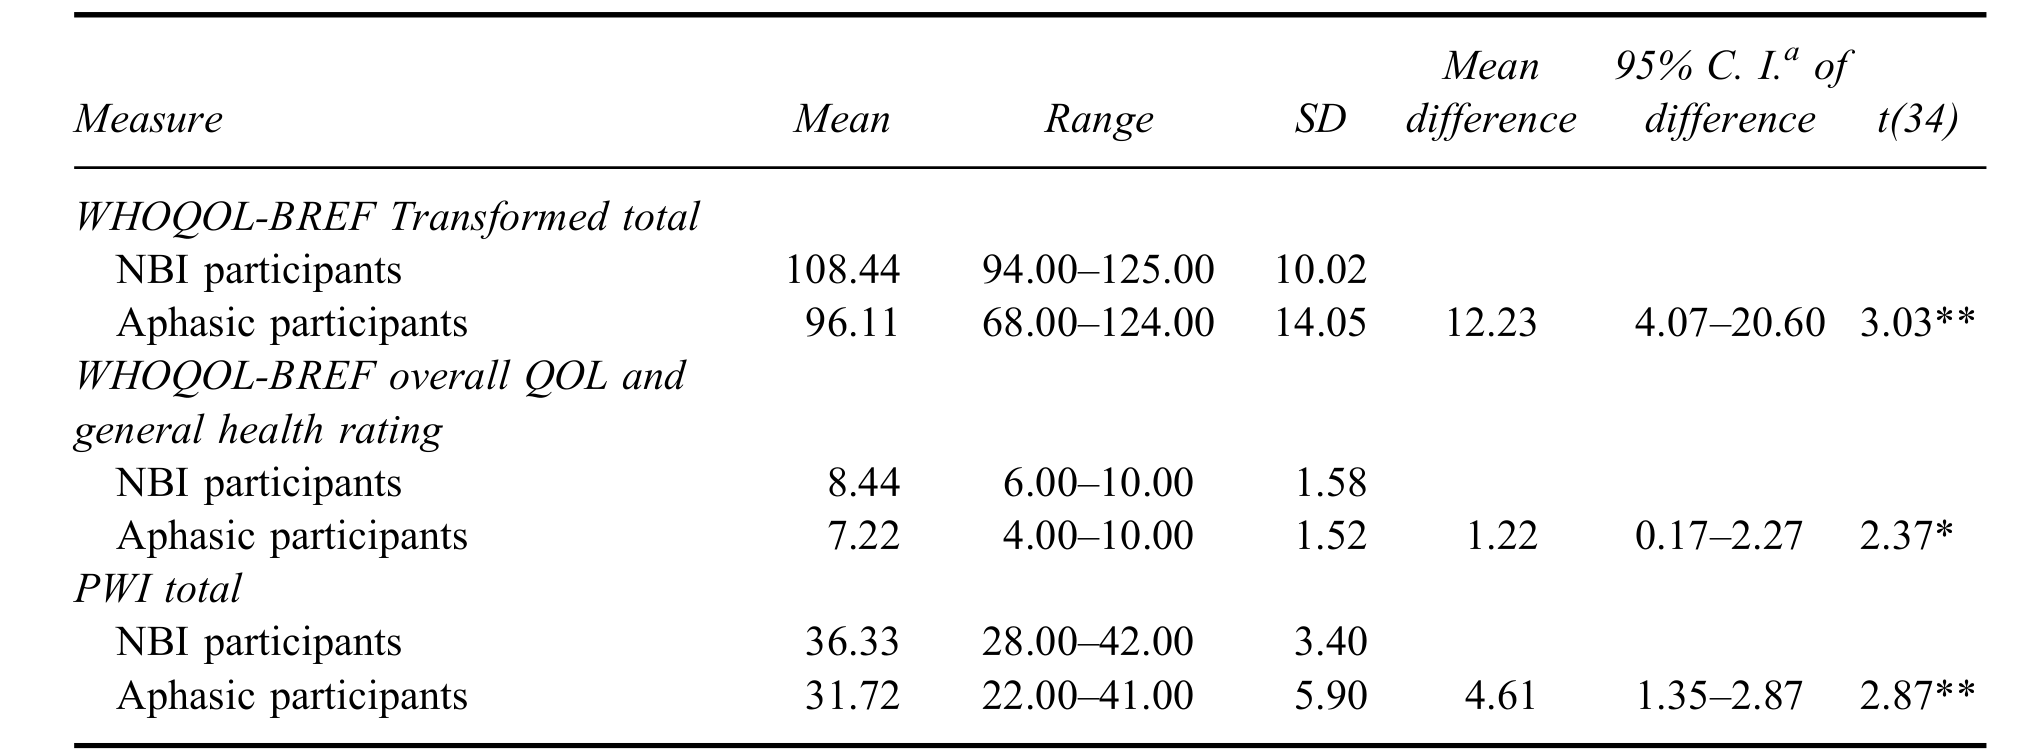
\includegraphics[width=12cm]{assets/images/qol.png}
    \caption[Comparaison de la qualité de vie chez les individus saints et ceux qui souffrent d'une aphasie.]%
    {Comparaison de la qualité de vie chez les individus saints et ceux qui souffrent d'une aphasie~\cite{Ross_Wertz_2010}.}
    \label{tab.qol-compare}
\end{table}



En particulier, l'aphasie de Broca diminue mesurablement la qualité de vie des individus qu'elle affecte
dans toute tâche qui nécessite la communication~\cite{Pallavi_Perumal_Krupa_2018}. 
La Table~\ref{fig.qocl-compare} le montre bien pour les trois exemples d'activités sociales, confiances en soi
et capacité à réaliser ses responsabilités quotidiennes.

\begin{figure}[hbt]
    \centering
    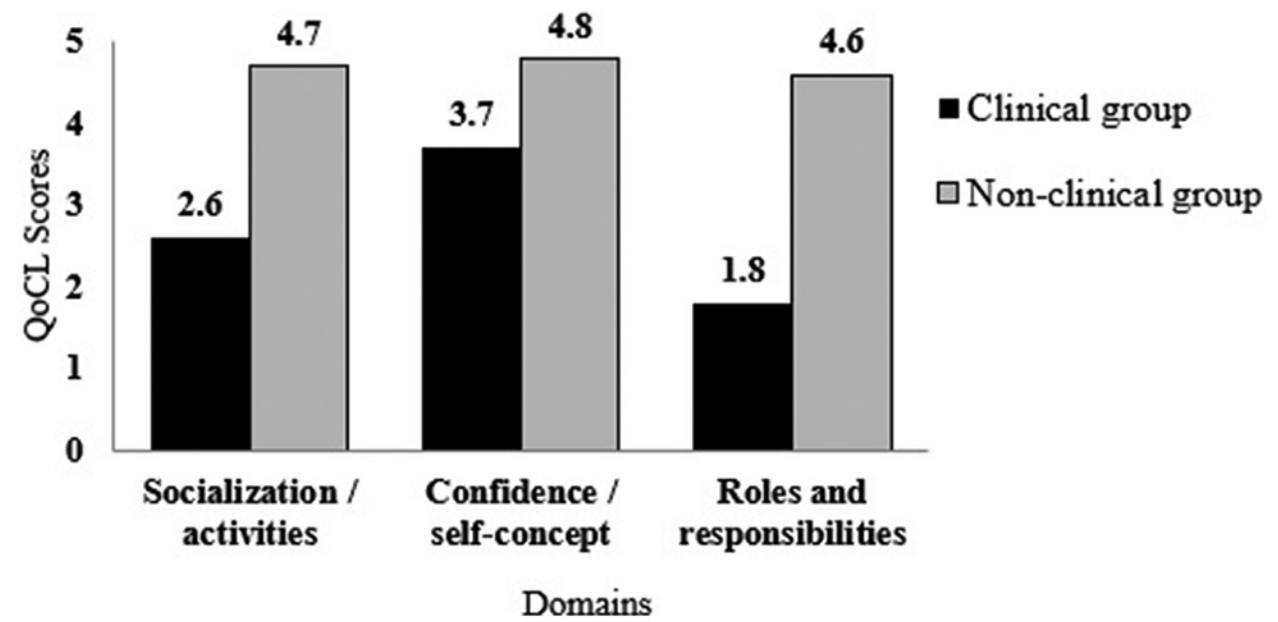
\includegraphics[width=10cm]{assets/images/qocl.png}
    \caption[Comparaison de la qualité de vie de communication chez les individus saints et ceux qui souffrent de l'aphasie de Broca.]%
    {Comparaison de la qualité de vie de communication chez les individus saints et ceux qui souffrent de l'aphasie de Broca~\cite{Pallavi_Perumal_Krupa_2018}.}
    \label{fig.qocl-compare}
\end{figure}
